\documentclass[10pt,twocolumn,letterpaper]{article}

\usepackage{cvpr}
\usepackage{times}
\usepackage{epsfig}
\usepackage{graphicx}
\usepackage{amsmath}
\usepackage{amssymb}
\usepackage{siunitx}
\usepackage{textcomp}
% Include other packages here, before hyperref.

% If you comment hyperref and then uncomment it, you should delete
% egpaper.aux before re-running latex.  (Or just hit 'q' on the first latex
% run, let it finish, and you should be clear).
\usepackage[pagebackref=true,breaklinks=true,letterpaper=true,colorlinks,bookmarks=false]{hyperref}
% \cvprfinalcopy % *** Uncomment this line for the final submission

\def\cvprPaperID{4263} % *** Enter the CVPR Paper ID here
\def\httilde{\mbox{\tt\raisebox{-.5ex}{\symbol{126}}}}

% Pages are numbered in submission mode, and unnumbered in camera-ready
\ifcvprfinal\pagestyle{empty}\fi
\begin{document}

%%%%%%%%% TITLE
\title{Layered Optical Flow Estimation using a soft-mask Module in Deep Neural Networks}

\author{First Author\\
Institution1\\
Institution1 address\\
{\tt\small firstauthor@i1.org}
% For a paper whose authors are all at the same institution,
% omit the following lines up until the closing ``}''.
% Additional authors and addresses can be added with ``\and'',
% just like the second author.
% To save space, use either the email address or home page, not both
\and
Second Author\\
Institution2\\
First line of institution2 address\\
{\tt\small secondauthor@i2.org}
}

\maketitle
%\thispagestyle{empty}

%%%%%%%%% ABSTRACT
\begin{abstract}
Using a layered representation for motion estimation has the advantage of being able to cope with discontinuities and occlusions. In this paper, we learn to estimate optical flow by combining a layered motion representation with deep learning. Instead of pre-segmenting the image to layers, the proposed approach automatically generates a layered representation of optical flow using the proposed soft-mask module. The essential components of the soft-mask module are maxout and  fuse operations, which enable a disjoint layered representation of optical flow and more accurate flow estimation. We show that by using masks the motion estimate results in a quadratic function of input features in the output layer. The proposed soft-mask module can be added to any existing optical flow estimation networks by replacing their flow output layer. In this work we use FlowNet as the base network to which we add the soft-mask module. The resulting network is tested on three well known benchmarks with both supervised and unsupervised flow estimation tasks. Evaluation results show that the proposed network achieve better results compared with respect to the original FlowNet. 
\end{abstract}

%%%%%%%%% BODY TEXT
\section{Introduction}
Optical flow estimation is a crucial and challenging problem which numerous applications in computer vision. Traditional differential methods for estimating optical flow include patch based methods, such as affine flow and Lucas-Kanade~\cite{Lucas:1981:IIR:1623264.1623280} and variational methods such as Horn and Schunck in~\cite{horn1981determining}. which includes a regularization term and provide a global solution of optical flow. Various of successful improvement of these initial formulations have been proposed over many years.

Layered models of optical flow offer an easy performance boost for optical flow estimation~\cite{wang1994representing}\cite{341161}\cite{darrell1995cooperative}. Disjointly splitting the optical flow into layers enables an easier modeling of optical flow in each layer. Such representation is especially helpful for small object motion estimation, as many optical flow estimation techniques are biased towards motion in large areas. Layered representation also improves flow computation on flow field boundaries by handling the smoothness constraint separately in each layer.

FlowNet proposed by Dosovitskiy~\cite{7410673} was the first work for use a deep neural network to end-to-end optical flow estimation. The concept of training FlowNet is fundamentally different from established differential approaches. As traditional differential optical flow estimation techniques perform well and are well established, several deep learning based approaches tried to bridge the gap between traditional approaches and deep learning based approaches by using the best on both sides. For example, Ranjan and Blacks~\cite{Ranjan_2017_CVPR} use a pyramid representation of flow and residual flows to address large flow displacement estimation. Several approaches~\cite{ren2017unsupervised}\cite{ahmadi2016unsupervised}\cite{DBLP:journals/corr/YuHD16} investigated the basic principles of flow estimation and proposed unsupervised training of networks.   

Our work combines the idea of using layered optical flow representation with a deep neural network structure. Unlike previous approaches~\cite{yang2015dense}\cite{black1996estimating}\cite{ju1996skin}, where the layered representation has was generated separately, the layered representation in the proposed approach is inferred internally and automatically when training the neural network. We achieve this by designing a soft-mask module. The soft-mask module is a network structure which splits optical flow to layers using disjoint real valued masks. As the masks are not binary we use the term 'soft' to refer to them. The soft-mask module offers a more accurate flow estimation due to two unique characteristics. The first is its ability to represent estimated flow using disjoint layers, which results in a more focused and simpler flow estimation for each layer. Second, compared with the linear flow output in FlowNet, the flow estimated using the soft-mask module is a quadratic in terms of input features, which allows the soft-mask module a better abilitys to fit more complicated optical flow patterns. The idea of using the soft-mask module is similar to maxout networks proposed by Goodfellow~\cite{Goodfellow:2013:MN:3042817.3043084}, where the output of a neuron is the max of a set of inputs. The proposed soft-mask module extends the maxout operation to 2D.  In addition, instead of keeping max value only, we zero-out non-max values and use these values as mask-out region when masks are fused with layered optical flows.

In this work, the soft-mask module is added to FlowNet by replacing the output layer of the network with the soft-mask module. More generally, the soft-mask module may be used in other per-pixel prediction tasks such as semantic segmentation~\cite{long2015fully} and single image depth estimation~\cite{eigen2014depth}. We that by using the soft-mask module we boost the performance of FlowNet when tested on several public datasets.  We further show that, both supervised and unsupervised flow estimation methods benefit from using the soft-mask module.

\subsection{Related Work}
Our work effectively combines ideas from using layered representation in classical optical flow approaches with recent deep learning approaches. Our literature review thus focuses on the work most relevant to this.
\newline
\newline
\noindent \textbf{Layered approaches.}
Using layered approaches in motion estimation have been demonstrated as an approach for motion estimation by using layers to overcome discontinuities and occlusions. A layered approach has been proposed by Darrell and Pentland~\cite{darrell1991robust}\cite{darrell1995cooperative} where they incorporate a Bayesian model for segmentation and robust statistics. Wang and Adelson~\cite{wang1993layered}\cite{wang1994representing} use affine layers to represent the motion field. Similarly, recent work by Sun \etal~\cite{sun2010layered}\cite{sun2012layered} use affine motion to regularize the flow in each layer, while Jepson and Black~\cite{341161} formalize the problem using probabilistic mixture models. Yang~\etal~\cite{yang2015dense} fit a piecewise adaptive flow field using piecewise parametric models while maintaining a global inter-piece flow continuity constraint. Exploiting recent advances in semantic scene segmentation, \cite{Sevilla-Lara_2016_CVPR} use different flow types for segmented object in different layers. Hur and Roth~\cite{Hur2016} treat semantic segmentation and flow estimation as a joint problem. Additional methods for joint motion and segmentation estimation includes~\cite{birchfield1999multiway}\cite{cremers2005motion}\cite{memin2002hierarchical}\cite{roussos2012dense}\cite{unger2012joint}\cite{yamaguchi2013robust}\cite{zitnick2005consistent}.
\newline
\newline
\noindent \textbf{Deep learning approaches.}
Deep neural networks have been shown to be successful in many computer vision tasks including object recognition~\cite{he2016deep} and dense prediction problems~\cite{zheng2015conditional}\cite{long2015fully}. FlowNet attempts to solve optical flow estimation using a deep neural network. FlowNet provides an end-to-end optical flow learning framework which serves as a base model for many later work~\cite{Ilg_2017_CVPR}\cite{ahmadi2016unsupervised}\cite{ren2017unsupervised}\cite{DBLP:journals/corr/YuHD16}



\subsection{Novel Contribution}
In this work, we extend FlowNet~\cite{7410673} to improve its performance in several ways. First, we propose to combine a traditional layered approach for optical flow estimation with deep learning. The proposed approach does not require pre-segmentation of images, instead, the separation of layers is automatically done when training the network. Second, a soft-mask module is proposed. This soft-mask module implements a channel-wise maxout operation among masks. As a result, the estimated optical flow will be separated to layers, each of which will contain optical flow that is estimated using a quadratic function. Third, we extend the FlowNet by adding the proposed soft-mask module in the output layers. The resulting network is trained and compared with both supervised and unsupervised optical flow estimation approaches using neural networks. Experimental results show that the proposed network structure achieves comparable or lower error in each experimental group.

\section{Methodology}
\subsection{Objective}
Given a pair of images $I_a, I_b \in \mathbb{R}^{H\times W\times C}$ as input, where $H, W$ and $C$ are height, width and channels of the input images, the proposed approach estimates an optical flow field $\bold{u}, \bold{v} \in \mathbb{R}^{H\times W}$, where $\bold{u}$ and $\bold{v}$ are the horizontal and vertical components of the optical flow field that transform image $I_a$ to image $I_b$. Following the optical flow objective by Horn and Schunck~\cite{horn1981determining}, which combines a data term enforcing the optical flow constraint equation and a regularization term enforcing smoothness. The classical optical flow objective thus is defined as:

\begin{equation}
\label{eqn: flow objective}
E(\bold{u}, \bold{v}) = \sum_{i}^H\sum_{j}^W (I_0(i+u_{ij}, j+v_{ij}) - I_1(i, j))^2 + 、\lambda \cdot \varphi(\bold{u, v})
\end{equation}
In this equation $\varphi(\bold{u}, \bold{v}))$ is a regularization term that constrains the smoothness of optical flow and $\lambda$ is a weight coefficient. 

The above objective is used by several deep neural network based for optical flow estimation based on an unsupervised training framework~\cite{ahmadi2016unsupervised}\cite{ren2017unsupervised}\cite{DBLP:journals/corr/YuHD16}. 

\begin{figure}[h]
\centerline{
\begin{tabular}{cc}
  \resizebox{0.089\textwidth}{!}{\rotatebox{0}{
  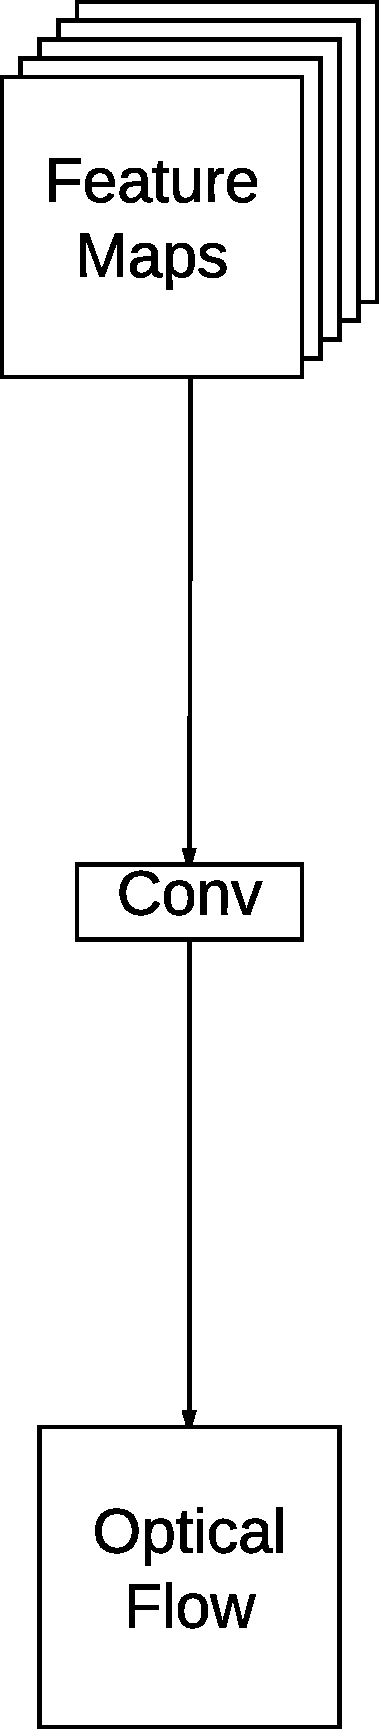
\includegraphics{Pic/PDF/NetworkStructure/Normal.pdf}}}
  &
  \resizebox{0.21\textwidth}{!}{\rotatebox{0}{
  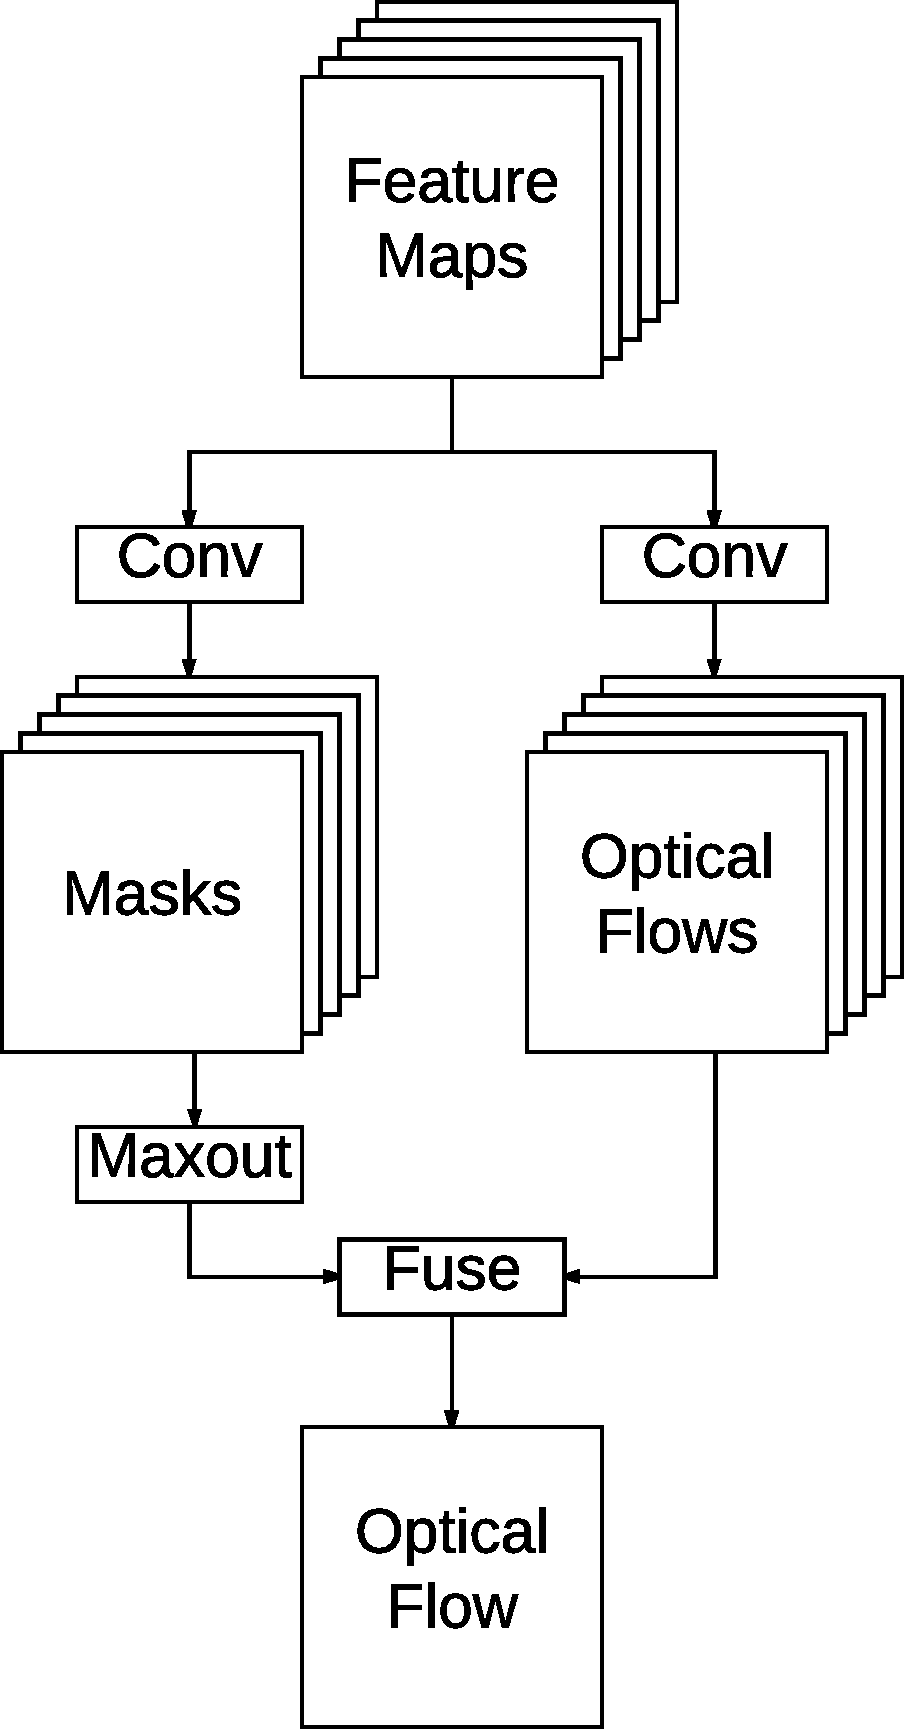
\includegraphics{Pic/PDF/NetworkStructure/MaskModule.pdf}}}
  \\
  a. Normal output & b. soft-mask module 
  \\
\end{tabular}}
\caption{Illustration of the structure of the proposed soft-mask module compared with traditional linear optical flow network.}
\label{fig: soft-mask module}
\end{figure} 

\subsection{soft-mask module}
FlowNet~\cite{7410673} was the first work to use deep convolutional neural network for optical flow estimation. The network architecture used by FlowNet is very similar to the structure of a classical auto-encoder, where optical flows are generated using deconvolution at each scale level of the image pyramid. To refine flow estimations, shortcuts are built to connect layers of corresponding levels in encoder and decoder layers. Consider a single computation of convolution, and for simplicity, assume that $f$ represents both horizontal and vertical components of an output flow. Given $X \in \mathbb{R}^{s\times s \times c}$, representing an input feature volume vector, where $s$ is kernel size and $c$ is number of channels, FlowNet employs a linear activation to compute optical flow:

\begin{equation}
f = X^T W + b
\end{equation}

\begin{figure}[h]
\centerline{
\begin{tabular}{c}
  \resizebox{0.25\textwidth}{!}{\rotatebox{0}{
  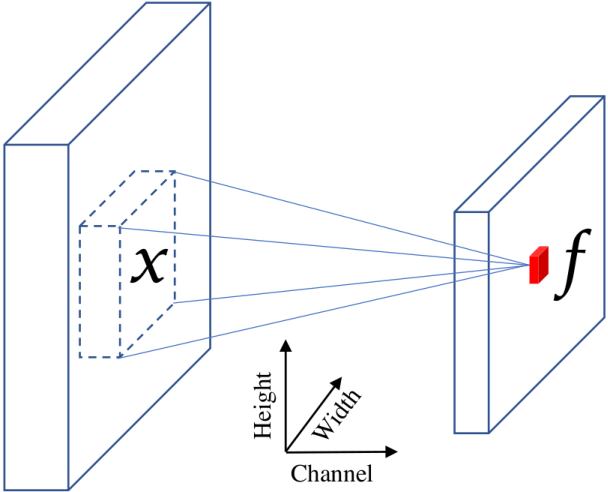
\includegraphics{Pic/PDF/conv_demo-crop.pdf}}}
  \\
\end{tabular}}
\caption{An illustration of annotation used in convolution.}
\label{fig: conv_layer}
\end{figure} 

Given that actual optical flow fields are nonlinear and piecewise smooth, using linear function to fit the flow field shifts non-linearity to the convolutional layers making the learning there more difficult. Using the soft-mask module proposed in this paper to replace the linear output of optical flow estimation, we are able to separate optical flow field to multiple layers. The flow estimation in each layer is smooth and is easier to estimate using a linear function. This results in a more accurate and flexible optical flow estimation. 

An illustration of the soft-mask module is shown in Figure~\ref{fig: soft-mask module}. The essential part of the soft-mask module is its dual-branch structure which contains a mask branch and an optical flow branch. The input feature maps represented as a set of volume feature vectors, $X \in \mathbb{R}^{s\times s \times c}$ are fed to both branches. The most significant contribution of this work is the separation of the optical flow field to multiple layers. For a separation into $k$ layers, $k$ masks will be generated in the mask branch as illustrated in Figure~\ref{fig: soft-mask module}. This requires $k$ convolutional filters $\{W_n^m, b_n^m\}_{n=1}^k$ in the mask branch. Correspondingly, the same number of filters are used in optical flow branch $\{W_n^f, b_n^f\}_{n=1}^k$. The mask and intermediate optical flow are then computed as follows:

\begin{align}
\label{eqn: computation of masks and flows}
m_n =& X^T W_n^m + b_n^m &\! \text{for $n = 1\dots k$} \nonumber\\
f_n =& X^T W_n^f + b_n^f &\! \text{for $n = 1\dots k$}
\end{align}
Thus, given $k$ filters, we will obtain $k$ corresponding pairs of mask and intermediate optical flow. By using $k$ filters in the optical flow branch and generating $k$ intermediate optical flow fields, we assume that each filter will work independently and model a single type or a few types of object motions. Correspondingly, filters in the mask branch are expected to mask out parts with consistent motions by being high in certain regions and low in others. This leads us to use a maxout operation to extract mask entries with maximal activation along the channel axis. After the maxout operation, for each mask $m_n (n=1\dots k)$, all entries will be zero-out except for entries whose activation values are maximal in the some region among all masks. We denote the masks after maxout using $\{m_n'\}_{n=1}^k$. Following the maxout operation, there is no intersection among masks and the union of all $m_n', n=1\dots k$ has activation in the full region. The maxout is given by:

\begin{equation}
\label{eqn: maxout}
m_n'=
\begin{cases}
m_n, & \text{if}\ m_n = \max\limits_{p=1\dots k}(m_p) \\
0, & \text{otherwise}
\end{cases} \quad \text{for $n = 1\dots k$}
\end{equation}

Note that, the masks after maxout are not converted to binary values. thus resulting in soft-masks. By using soft masks we are able to not only mask out irrelevant parts, but also prioritize values in each layer.

\begin{figure}[h]
\centerline{
\begin{tabular}{c}
  \resizebox{0.45\textwidth}{!}{\rotatebox{0}{
  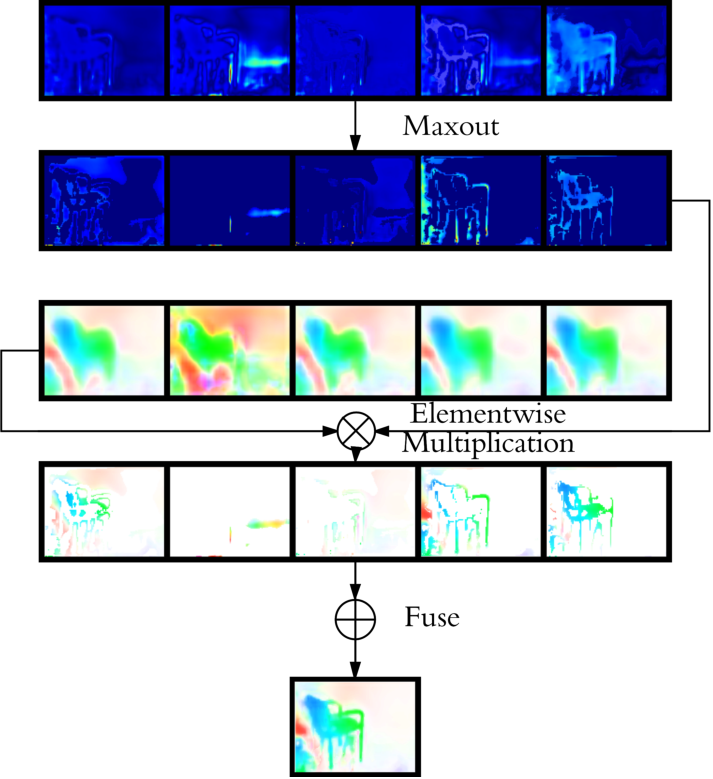
\includegraphics{Pic/PDF/Pipeline.pdf}}}
  \\
\end{tabular}}
\caption{Pipeline of soft-mask module.}
\label{fig: softmask pipeline}
\end{figure} 

In the proposed approach, masks after the maxout operation are applied to corresponding intermediate optical flow field by element-wise multiplication as shown below:

\begin{figure*}[th]
\centerline{
\begin{tabular}{c}
  \resizebox{0.92\textwidth}{!}{\rotatebox{0}{
  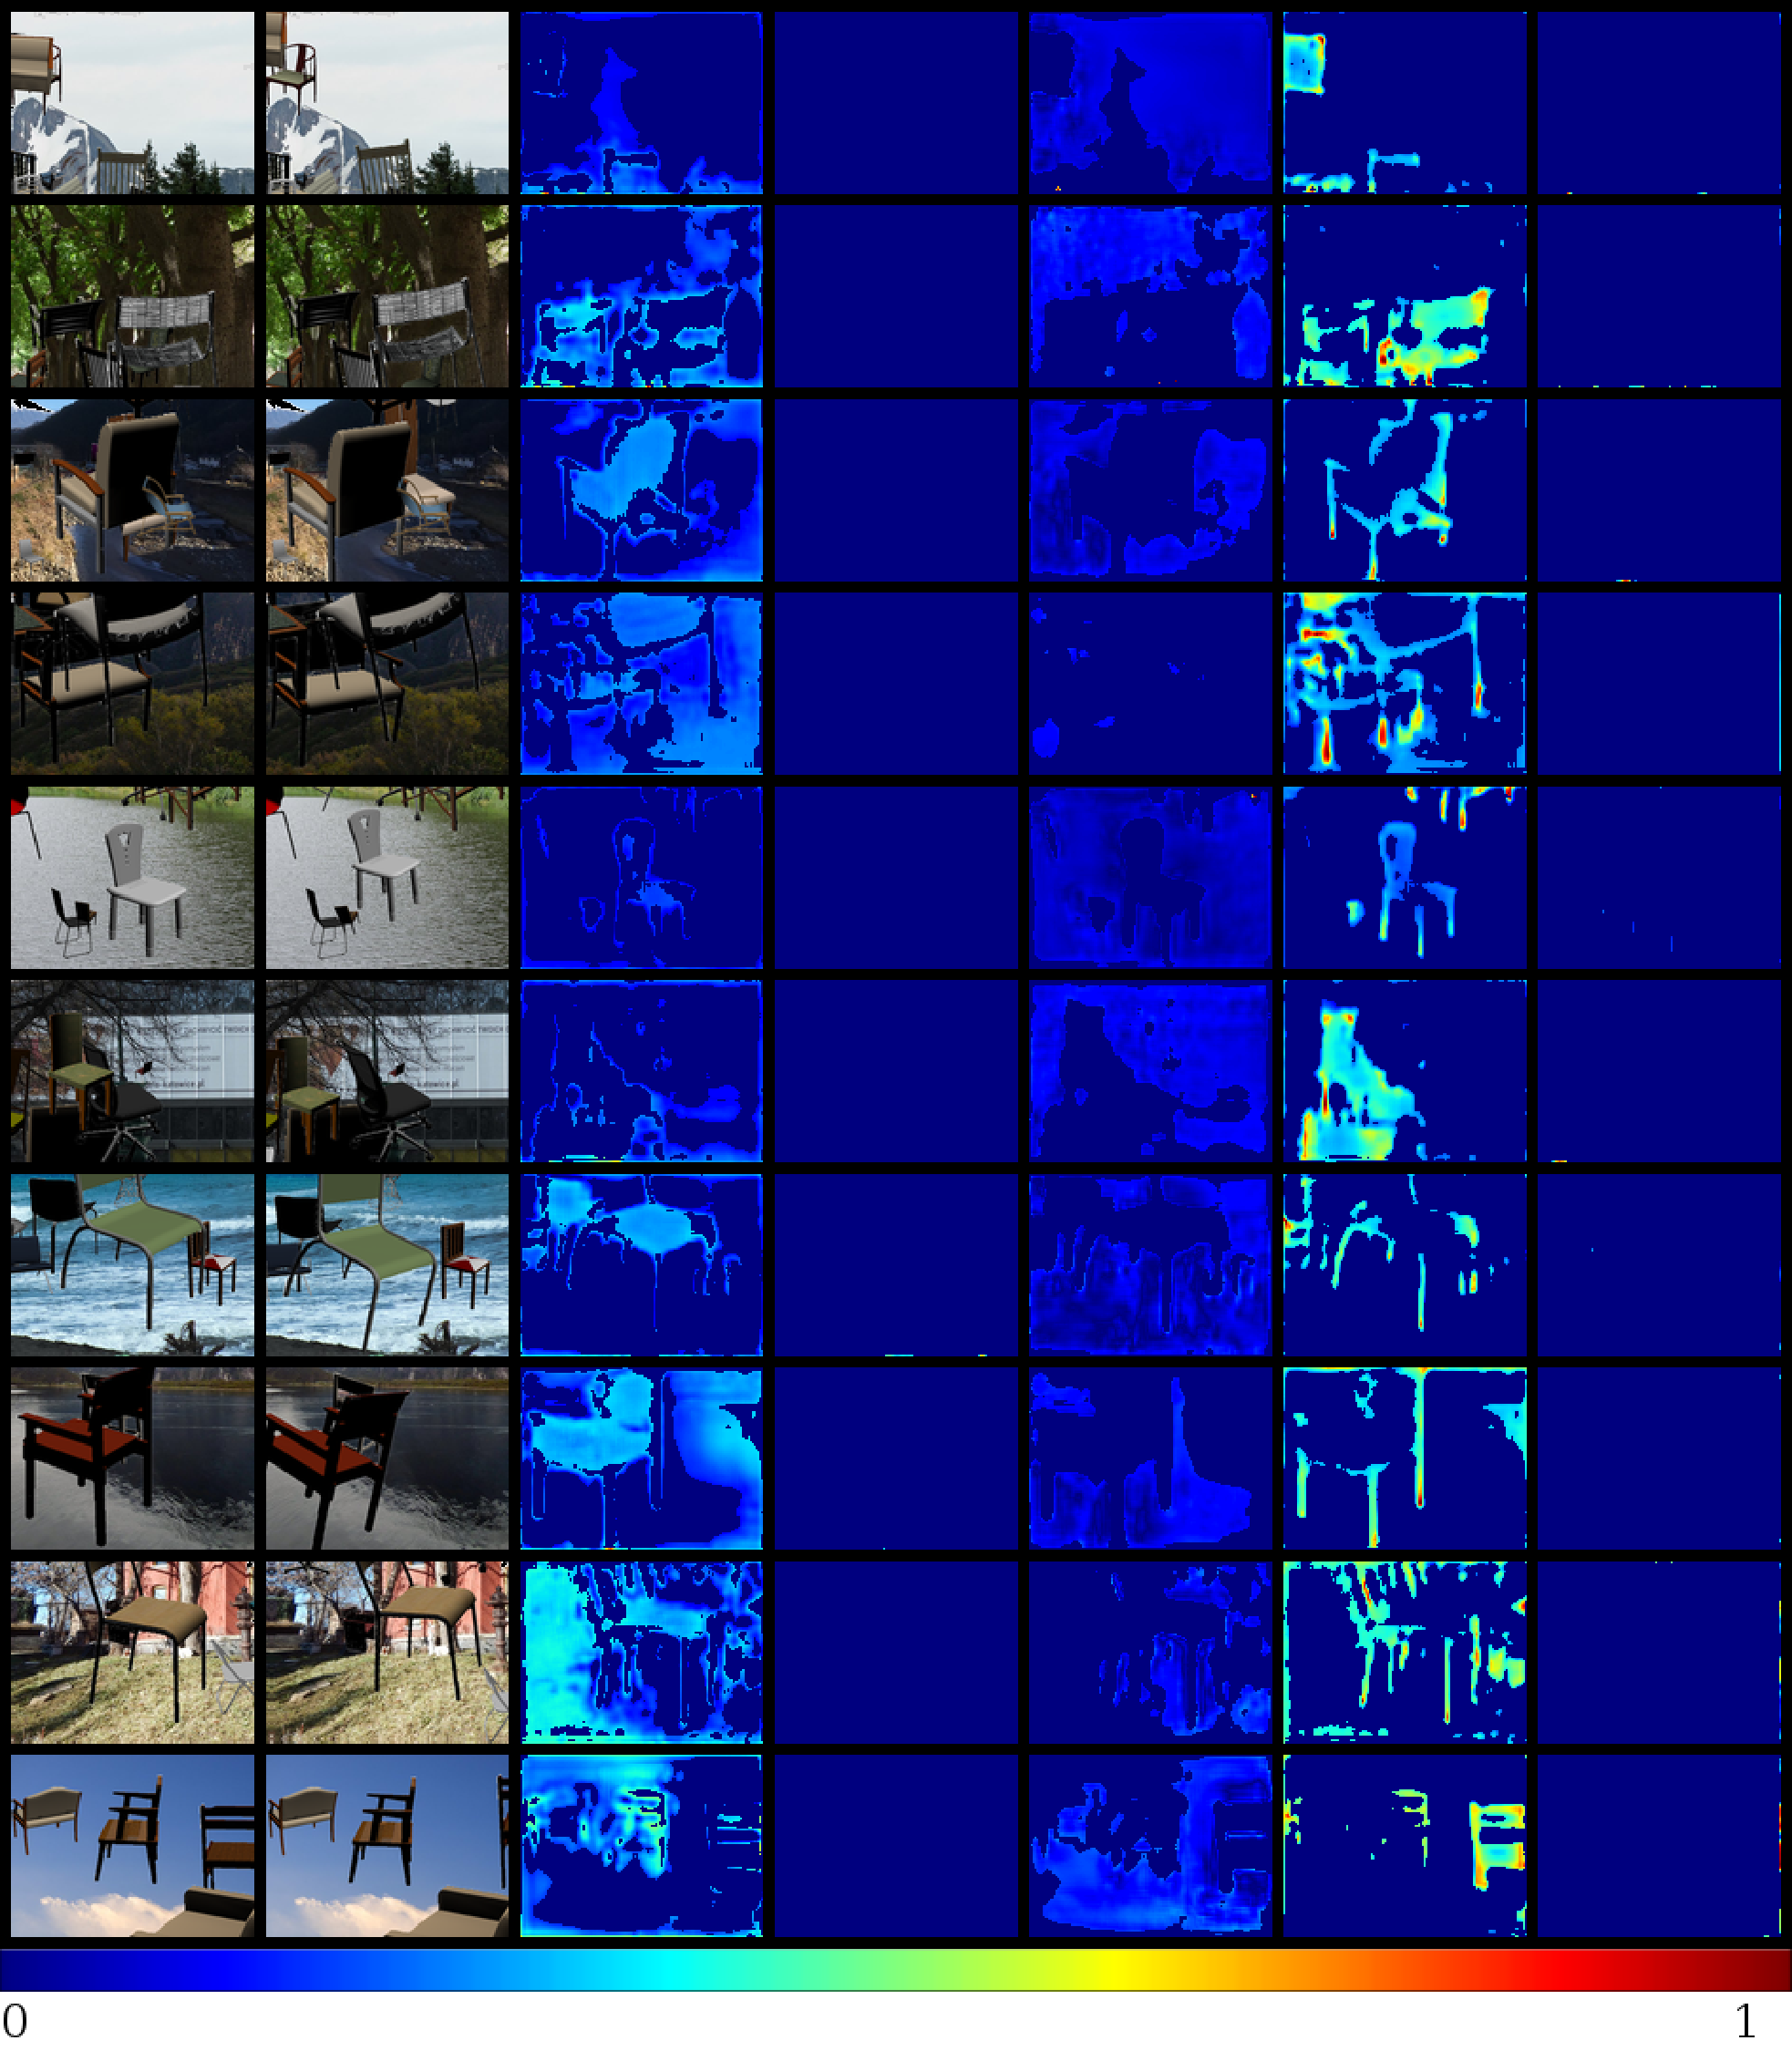
\includegraphics{Pic/PDF/Masks_demo.pdf}}}
  \\
\end{tabular}}
\caption{Examples of generated masks using the proposed soft-mask module. In this example, five masks are generated for each input image pair (left). Note that column 4 and 7 are not empty. Some small structures such as flows on the boundaries are captured by masks in these two columns. The rendering of the figure is best viewed electronically.}
\label{fig: maxout demo}
\end{figure*} 

\begin{equation}
\label{eqn: maxout}
f_n'=
\begin{cases}
m_n' \times f_n, & \text{if}\ m_n' \neq 0 \\
0, & \text{otherwise}
\end{cases} \quad \text{for $n = 1\dots k$}
\end{equation}
The results of the above computation is a set of disjoint optical flow layers, each of which represents a certain type of motion. An illustration of how the soft-mask module works is show in Figure~\ref{fig: softmask pipeline} and results of generated masks are shown in Figure~\ref{fig: maxout demo}.



\subsection{Quadratic fitting of optical flow}
Objects move in different ways, which results in different types of motion. The underlying optical flows thus are non-linear and locally piece-wise smooth. 

There are two consequences of using the proposed soft-mask module that could make the estimation of the optical flow easier. The first advantage of using the soft-mask module originates from using maxout in mask generation. By keeping only the maximal value among all masks, the optical flow is separated to multiple disjoint layers. Theoretically proving that maxout result in a precise cut along motion boundaries is challenging and is still under investigation. However, qualitative results as shown in Figure~\ref{fig: maxout demo} demonstrate that the soft-mask module enable resulting masks to separate the flow field into pieces according to detected motion types. In addition, the masks detect the boundary of each piece, which allows for the estimation of optical flows on boundaries to be more accurate.  The second advantage of using the proposed soft-mask module is that the output is quadratic in terms of feature maps $X$ fed to the module. To see this, consider the computation of masks and intermediate optical flows shown in Equation~\ref{eqn: computation of masks and flows}. The computation of non-zero $f_n'$ could be written as:

\begin{align}
f_n' & = m_n' \times f_n \nonumber\\
	 & = (X^T W_n^m + b_n^m) \times (X^T W_n^f + b_n^f) \nonumber\\
	 & = W_n^{mT} X X^T W_n^f + X^T(b_n^f W_n^m + b_n^m W_n^f) + b_n^m b_n^f
\end{align}
As shown in the above equation, the representation of $f_n'$ is quadratic in terms of the variable $X$.

To better illustrate the advantage in using the soft-mask module with respect to linear output. Consider the 1D example shown in Figure~\ref{fig: quadratic demo}. In this example, function values are smooth in three separate domains. The improvement of fitting data using a piecewise quadratic function is shown by comparing B and C.

\begin{figure}[h]
\centerline{
\begin{tabular}{ccc}
  \resizebox{0.15\textwidth}{!}{\rotatebox{0}{
  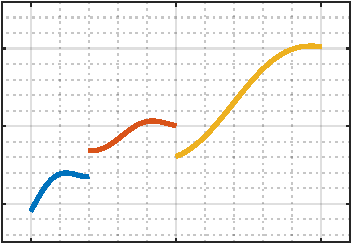
\includegraphics{Pic/PDF/QuadraticFuncDemo/FitDemo_1-crop.pdf}}}
  &
  \resizebox{0.15\textwidth}{!}{\rotatebox{0}{
  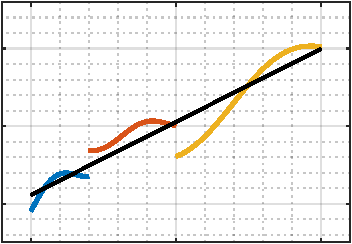
\includegraphics{Pic/PDF/QuadraticFuncDemo/FitDemo_2-crop.pdf}}}
  &
  \resizebox{0.15\textwidth}{!}{\rotatebox{0}{
  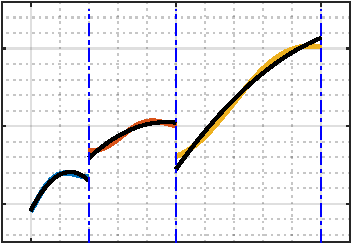
\includegraphics{Pic/PDF/QuadraticFuncDemo/FitDemo_3-crop.pdf}}}
  \\
  A & B & C
  \\
\end{tabular}}
\caption{A: Given data. B: Fitting using linear function. C: Fitting using piecewise quadratic function.}
\label{fig: quadratic demo}
\end{figure} 

\subsection{Regularization for Unsupervised Training}
Training an unsupervised neural network for optical flow estimation is possible by using a network similar to FlowNet for base optical flow inference followed by a spatial transform network (STN)~\cite{jaderberg2015spatial} to generate warped iamges for comparison. Existing work such as: DSTFlow~\cite{ren2017unsupervised}, USCNN~\cite{ahmadi2016unsupervised}, and back-to-basic unsupervised FlowNet (bb-FlowNet)~\cite{DBLP:journals/corr/YuHD16} all follow the same framework and train their networks without supervision to minimize the objective defined in Equation~\ref{eqn: flow objective}.  To show that proposed soft-mask module can improve flow estimation using the same framework, we add the soft-mask module to FlowNet and use it as a base optical flow inference network in an unsupervised training framework.

The smoothness term which is used by all above unsupervised approaches plays a significant role in regularizing the local consistancy of optical flow. We use the bending energy regularization~\cite{rohlfing2003volume}\cite{ashburner1999nonlinear} defined by:

\begin{align*}
\varphi(\bold{u}, \bold{v}) = & \sum ((\frac{\partial^2\bold{u}}{\partial \bold{x}^2})^2+(\frac{\partial^2\bold{u}}{\partial \bold{y}^2})^2+2(\frac{\partial^2\bold{u}}{\partial \bold{x} \partial \bold{y}})^2) + \\ 
& \sum ((\frac{\partial^2\bold{v}}{\partial \bold{x}^2})^2+(\frac{\partial^2\bold{v}}{\partial \bold{y}^2})^2+2(\frac{\partial^2\bold{v}}{\partial \bold{x} \partial \bold{y}})^2)
\end{align*}


\section{Empirical Evaluation}
\label{sec: evaluation}
\subsection{Benchmark}
We evaluate our performance on three standard optical flow benchmarks: Flying Chairs~\cite{7410673},  Sintel~\cite{Butler:ECCV:2012}, and KITTI~\cite{geiger2012we}. We compare the performance of the proposed approach to both supervised methods such as: FlowNet(S/C)~\cite{7410673}, SPyNet~\cite{Ranjan_2017_CVPR}, DeepFlow~\cite{weinzaepfel2013deepflow}, and EpicFlow~\cite{revaud2015epicflow}, and  unsupervised methods including: DSTFlow~\cite{ren2017unsupervised}, USCNN~\cite{ahmadi2016unsupervised}, and back-to-basic unsupervised FlowNet (bb-FlowNet)~\cite{DBLP:journals/corr/YuHD16}. 

Recently, FlowNet 2.0, a follow-up work of FlowNet, achieved state of the art results on most datasets. The architecture of FlowNet 2.0~\cite{Ilg_2017_CVPR} uses several FlowNets and contains cascade training of the FlowNets in different phases. Since the focus of this paper is on using the soft-mask module to boost performance of a single network, we do not include FlowNet 2.0 in our evaluation. Note that the proposed soft-mask module can be incorporated into FlowNet 2.0.

\subsection{Network Structures}
The goal of this paper is to show how the performance of existing optical flow networks can be improved by replacing the normal optical flow output layer with the proposed soft-mask module. We choose FlowNetS and FlowNetC as the base networks and replace their optical flow output layers with a soft-mask module. Using the layered optical flow estimation (LOFE) proposed in this paper, we term the resulting modified networks: FlowNetS+LOFE and FlowNetC+LOFE, respectively. 

While we evaluate FlowNet in this work, the soft-mask module can be added to other networks and used on various vision tasks such as image segmentation~\cite{long2015fully}\cite{noh2015learning} and depth estimation in range images~\cite{eigen2014depth}\cite{eigen2015predicting}.

\subsection{Training Details}
Both supervised and unsupervised networks are trained using Adam~\cite{kingma2014adam} optimization with $\beta_1=0.9$ and $\beta_2=0.999$. We use a small batch size of 8 across all dataset with 3000 iterations per epoch. The initial learning rate is set to be $(1e-4)$ and decrease to half every 60 epochs until the network converge. All experiments were finished on a single Nvidia 1080 GPU.

Various types of data augmentation are used during training. We apply rotation at random within $[\ang{-17}, \ang{17}]$. A random translation within $[-50, 50]$ pixels is applied to both horizontal and vertical directions. In addition, following~\cite{Ranjan_2017_CVPR} we include additive white Gaussian noise sampled uniformly from $\mathcal{N}(0, 0.1)$. We also apply color jitter with additive brightness, contrast and saturation samlped from a Gaussian, $\mathcal{N}(0, 0.4)$. All data augmentation are done using GPU during training.

\begin{figure*}[th]
\centerline{
\begin{tabular}{c}
  \resizebox{0.95\textwidth}{!}{\rotatebox{0}{
  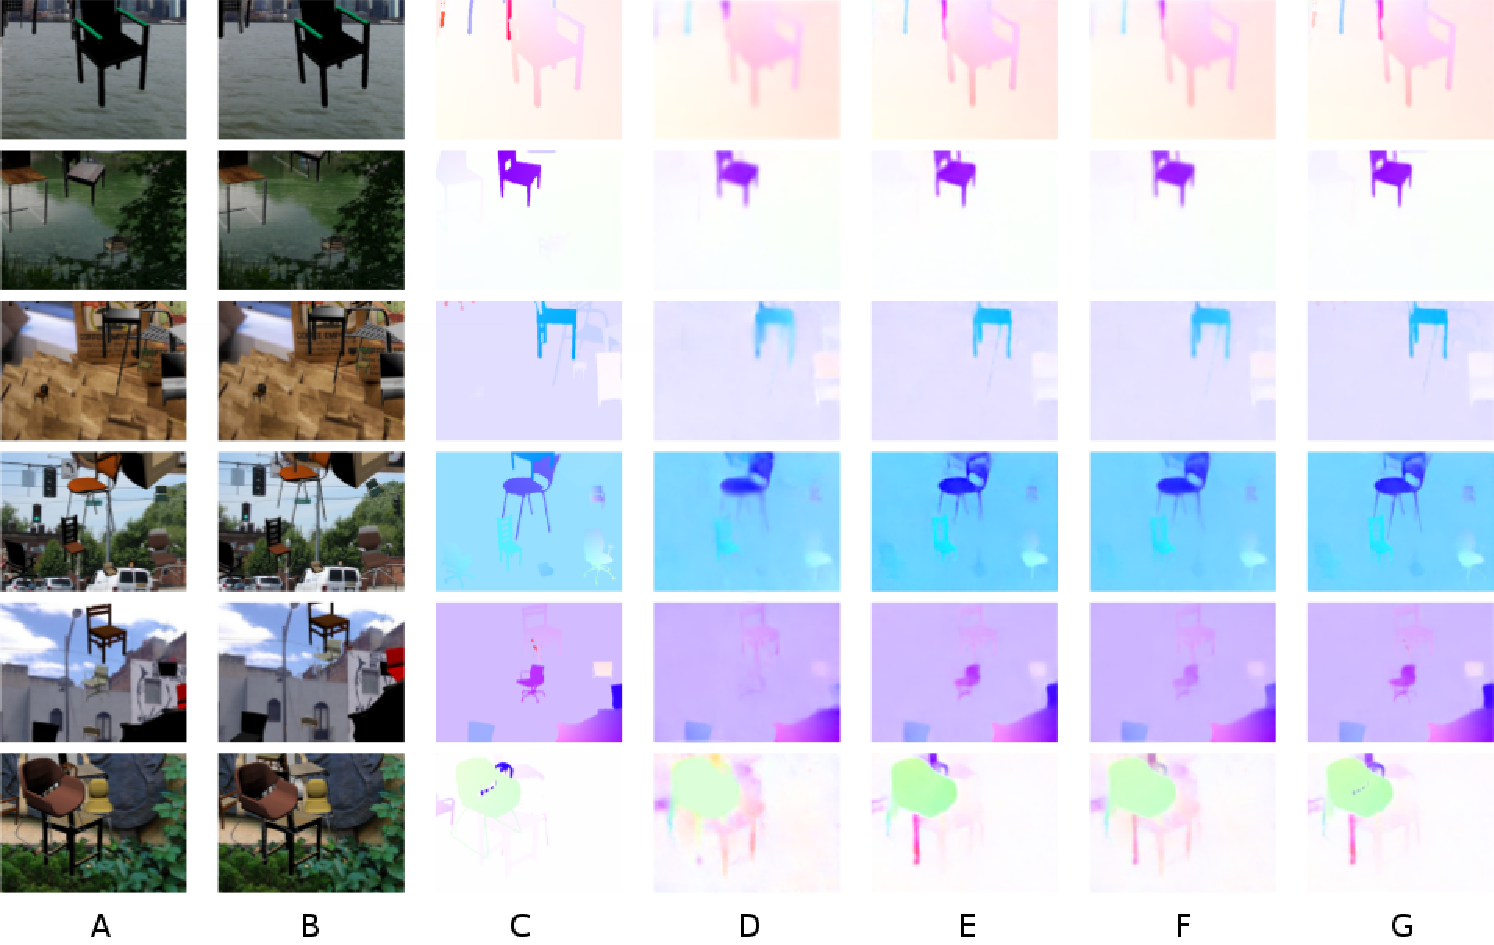
\includegraphics{Pic/PDF/Predictions/predictedflows.pdf}}}
  \\
\end{tabular}}
\caption{Examples of predicted flows compared with results from FlowNet. A/B: input image pairs. C: FlowNetS, D: FlowNetC, E: FlowNetS+LOFE, F: FlowNetC+LOFE.}
\label{fig: predicted flows}
\end{figure*} 

\subsection{Results}
Evaluations were done with compared methods in two groups according to whether the training of the methods is unsupervised or supervised. Table~\ref{tab: results supervised} shows the endpoint error (EPE) of the proposed network and several well known methods. The endpoint error measures the distance in pixels between known optical flow vectors and estimated ones. Except for EpicFlow and DeepFlow, all the other methods were trained in a supervised manner. We compare results of unsupervised methods in Table~\ref{tab: results unsupervised}.Note that FlowNet~\cite{Ilg_2017_CVPR} and SPyNet~\cite{Ranjan_2017_CVPR}, report additional fine-tuned network results which are not used here since we are interested in evaluating the impact of using the soft-mask module, and since fine tuning may vary between methods and thus mask differences.
\newline
\newline
\noindent \textbf{Supervised methods.} The proposed FlowNetS+LOFE and FlowNetC+LOFE tested in this group use $k=10$ for the number of layers. As can be seen from Table~\ref{tab: results supervised}, FlowNetS+LOFE and FlowNetC+LOFE achieve the best performance on all tests except for the training set of the Sintel Clean dataset. We observe that, the performance of FlowNetS and FlowNetC are both boosted by replacing the optical flow output layer with the soft-mask module. Considering the computation time we observe a small time increment when using the soft-mask module, and which is in an acceptable range. 
\newline
\newline
\noindent \textbf{Unsupervised methods.} Training optical flow estimation networks without supervision is straight forward by using the objective shown in Equation~\ref{eqn: flow objective}. The difficult part is to decide the weight coefficient $\lambda$ in the equation. To choose an appropriate $\lambda$, we did a grid search for the best value in a range of $[0, 10]$. We stopped the search when the improvement is small. The results are shown in Table\ref{tab: results unsupervised}. As can be observed, the proposed networks achieve the best performance except for KITTI dataset. 

\begin{table*}[]
\centering
\caption{Average end point errors (EPE) of the proposed networks compared to several existing methods. EpicFlow and DeepFlow are traditional methods which do not use neural networks. All other methods in the table are trained with supervised data. Bold font indicates the most accurate results among the network based methods.}
\label{tab: results supervised}
\begin{tabular}{lcccccccc}
\hline
\hline
\multicolumn{1}{c}{Method} & Flying Chairs & \multicolumn{2}{c}{Sintel Clean} & \multicolumn{2}{c}{Sintel Final} & \multicolumn{2}{c}{KITTI} & Time (s) \\
                           & Test          & Train           & Test           & Train           & Test           & Train            & Test   &          \\ \hline
EpicFlow                   & 2.94          & 2.40            & 4.12           & 3.7             & 6.29           & 3.47             & 3.8    & 16       \\
DeepFlow                   & 3.53          & 3.31            & 5.38           & 4.56            & 7.21           & 4.58             & 5.8    & 17       \\ \hline
FlowNetS                   & 2.71          & 4.50            & 7.42           & 5.45            & 8.43           & 8.26             & -      & 0.12     \\
FlowNetC                   & 2.19          & 4.31            & 7.28           & 5.87            & 8.81           & 9.35             & -      & 0.23     \\
SPyNet                     & 2.63          & \textbf{4.23}   & \textbf{6.82}           & 5.67            & 8.49           & 9.12             & -      & 0.11     \\
FlowNetS+LOFE              & 2.53          & 4.35            & 7.11           & \textbf{5.32}   & \textbf{8.25}  & \textbf{8.03}    & -      & 0.17     \\
FlowNetC+LOFE              & \textbf{2.08} & \textbf{4.23}            & 7.01  & 5.51            & 8.51           & 9.14             & -      & 0.30     \\ \hline
\end{tabular}
\end{table*}

\begin{table*}[]
\centering
\caption{EPE errors of methods that are trained without supervision. The results of compared methods are taken directly from the corresponding paper.}
\label{tab: results unsupervised}
\begin{tabular}{lccccccc}
\hline
\hline
\multicolumn{1}{c}{Method} & Flying Chairs & \multicolumn{2}{c}{Sintel Clean} & \multicolumn{2}{c}{Sintel Final} & \multicolumn{2}{c}{KITTI}      \\
                           &               & Train           & Test           & Train          & Test            & Train          & Test          \\ \hline
DSTFlow                    & 5.11          & 6.93            & 10.40          & 7.82           & 11.11           & \textbf{10.43} & -             \\
USCNN                      & -             & -               & -              & 8.88           & -               & -              & -             \\
BB-FlowNet                 & 5.36          & -               & -              & -              & -               & 11.32          & \textbf{9.93} \\
FlowNetS+LOFE              & \textbf{4.81} & \textbf{6.56}   & 10.10          & \textbf{7.62}  & 10.98           & 10.78          & 10.82         \\
FlowNetC+LOFE              & 4.92          & 6.78            & \textbf{9.98}  & 7.77           & \textbf{10.19}  & 11.01          & 11.25         \\ \hline
\end{tabular}
\end{table*}

\subsection{Evaluation of the soft-mask Module}
Since we replaced the simple linear output layer in FlowNet(S/C) with a more complex soft-mask module, we would like to verify whether the improved results are obtained due to the way then soft-mask module works and not simply due to having a model with more coefficients. To better investigate the operation of the soft-mask module, we compared the FlowNetC+LOFE with two other networks in which we slightly changed the structures of the soft-mask module.

In the first network, given the proposed structure as FlowNetC+LOFE, we removed the maxout operation from the soft-mask module and kept the remaining configuration the same. We denote the resulting work FlowNetC+LOFE/no-maxout. In this case FlowNetC+LOFE/no-maxout will have the exact same number of coefficients as FlowNetC+LOFE. For the second network, we  removed the mask branch from soft-mask module leaving only the intermediate optical flow only. The second network is denoted as FlowNetC+LOFE/no-masks. For all three networks, we use $k=10$ in the soft-mask module. We use original FlowNetC as a baseline in this comparison. In order to obtain an unbiased comparison result, we trained and tested each of these networks on the Flying Chairs dataset five times. The average EPE and standard deviation is reported in Table~\ref{tab: flownet variants}.

\begin{table}[]
\centering
\caption{Comparison of the proposed FlowNet+LOFE and its two variants.}
\label{tab: flownet variants}
\begin{tabular}{lc}
\hline
\hline
                         & Flying Chairs \\ \hline
FlowNetC                 & 2.19 $\pm$ 0.021            \\
FlowNetC+LOFE            & 2.08 $\pm$ 0.018            \\
FlowNetC+LOFE/no-maxout  & 2.16 $\pm$ 0.021            \\
FlowNetC+LOFE/no-masks   & 2.22 $\pm$ 0.021            \\
\hline
\end{tabular}
\end{table}

As can be seen from Table~\ref{tab: flownet variants}, the proposed FlowNet+LOFE performed better than its two variants. This comparison leads to two conclusions. First, the better performance obtained by adding the soft-mask module to FlowNet is not because a larger model being used. This is since the no-maxout version of the proposed network has identical complexity to the proposed network. Thus we conclude that the maxout operation make optical flow estimation an easier task by separating optical flows to different layers. Second, it can be seen from the table that the performance of the no-maxout version is slightly better than that of the no-masks version. While a possible explanation is that the model of no-maxout is bigger than the model of no-masks, note that FlowNet, the smallest model in this comparison, achieved a better performance than the no-masks model. We hypothesize that the reason leading to this result is a fact that the no-maxout version of model is using a quadratic function to fit optical flow instead of the linear function used by the no-masks version. 

\begin{figure}[th]
\centerline{
\begin{tabular}{c}
  \resizebox{0.48\textwidth}{!}{\rotatebox{0}{
  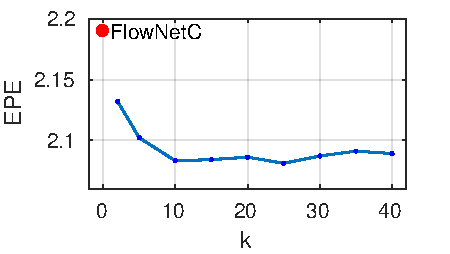
\includegraphics{Pic/PDF/k/K_Demo.pdf}}}
  \\
\end{tabular}}
\caption{EPE as a function of $k$, the number of layers used in soft-mask module.}
\label{fig: evaluation k}
\end{figure} 

We investigate the relationship between $k$ the number of masks and flow layers used in the soft-mask module, and network performance in terms of EPE. Experiments were done using the Flying Chairs dataset. We start with a soft-mask module with $k=2$, then set $k=5\mathrm{x}$, where $\mathrm{x}=1, \dots, 8$. As can be observed in Figure~\ref{fig: evaluation k}, there is an immediate benefit to using the soft-mask module with respect to FlowNetC, where $k=2$ will efficiently boost  performance. We see in Figure~\ref{fig: evaluation k} convergence after $k=10$ and a slightly increase when $k>25$. This may be due to slight overfitting when separating the optical flow to too many layers.



\section{Conclusion}
We describe a new approach for optical flow estimation by combining traditional layered flow representation with deep learning method. rather than pre-segmenting images to layers, the proposed approach automatically learns a layered representation of optical flow using the proposed soft-mask module. The soft-mask module has the advantage of splitting flow to layers in which the computation of the flow is quadratic in terms of input features. For evaluation, we use FlowNet as our base net to add the soft-mask module. The resulting networks are tested on three well known benchmark with both supervised and unsupervised flow estimation tasks. Experimental results show that the proposed network achieve better results with respect to the original FlowNet. 


{\small
\bibliographystyle{ieee}
\bibliography{mybib}
}

\end{document}
